\documentclass[twoside]{article}

\usepackage[sc]{mathpazo} 
\usepackage[spanish, es-tabla]{babel}
\usepackage[utf8]{inputenc}

\usepackage[hmarginratio=1:1,top=32mm,columnsep=20pt]{geometry} % Document margins
\usepackage{multicol} % Used for the two-column layout of the document
\usepackage[hang, small,labelfont=bf,up,textfont=it,up]{caption} % Custom captions under/above floats in tables or figures
\usepackage{mathtools}
\usepackage{float} % Required for tables and figures in the multi-column environment - [H] needed
\usepackage{hyperref} % For hyperlinks in the PDF with labels

\usepackage{abstract} % Allows abstract customization
\renewcommand{\abstractnamefont}{\normalfont\bfseries} % Set the "Abstract" text to bold
\renewcommand{\abstracttextfont}{\normalfont\small\itshape} % Set the abstract itself to small italic text

\usepackage{titlesec} % Allows customization of titles

\titleformat{\section}[block]{\large\scshape\centering}{\thesection.}{1em}{} % Change the look of the section titles
\titleformat{\subsection}[block]{\large\centering}{\thesubsection.}{1em}{} % Change the look of the section titles

\usepackage{fancyhdr} % Headers and footers
\pagestyle{fancy} % All pages have headers and footers
\fancyhead{} % Blank out the default header
\fancyfoot{} % Blank out the default footer
\fancyhead[C]{Resonadores Ópticos% based on TRACS 
\hspace{4pt} $\bullet$ \hspace{4pt} Noviembre 2018 } % Custom header text
\fancyfoot[RO,LE]{\thepage} % Custom footer text

%----------------------------------------------------------------------------
%	   TITLE SECTION
%----------------------------------------------------------------------------

\title{
	\vspace{-15mm}
	\fontsize{28pt}{10pt}
	\selectfont\textbf{Estudio de los Resonadores Ópticos}% Article title
}

\author{
	\large
	\textsc{Jaime D\'iez Gonz\'alez-Pardo}\\[4mm]
	\fontsize{28pt}{10pt} Universidad de Cantabria \\ % Your institution
	%\thanks{A thank you or further information}\\[2mm] % Your name
	\normalsize Fotónica \\ 
	%\normalsize{Compañeros:} \textsc{NOMBRE COMPANEROS }\\%\normalsize \href{mailto:john@smith.com}{john@smith.com} % Your email address
	%\vspace{5mm}
}

\date{ 13 de Noviembre de 2018 }


%----------------------------------------------------------------------------
%      · DOCUMENT
%----------------------------------------------------------------------------

\begin{document}


	\maketitle % Insert title


	\thispagestyle{fancy} % All pages have headers and footers

%----------------------------------------------------------------------------
%	  ABSTRACT
%----------------------------------------------------------------------------

	%\begin{abstract}

		%\noindent% Dummy abstract text

			%TEXTO RESUMEN

	%\end{abstract}

%----------------------------------------------------------------------------
%	  ARTICLE CONTENTS
%----------------------------------------------------------------------------

	\begin{multicols}{2} % Two-column layout throughout the main article text

		\section{Introducción} % Scope of the project = rad effects + minimization
							 
			Un resonador óptico es un dispositivo que consta de una cavidad sobre la que se incide luz con una cierta frecuencia de tal forma que dicha luz permanece confinada entre sus caras, produciendo una resonancia. El perfil del campo electromagnético en el plano transversal a la dirección de propagación del campo se denomina modo transversal electromagnético (TEM). En dichos modos no se tiene ninguna componente en la dirección de propagación del campo eléctrico o magnético. Si el lado de las superficies en las que se producen la resonancia es mucho menor que la longitud del resonador $L$, existe una diferencia entre los modos longitudinales de la forma:

				\begin{equation}
					\Delta \omega_L = \frac{\pi c}{L}
					\label{eq:long}
				\end{equation}

			Donde $c$ es la velocidad de la luz en el vacio.

			La diferencia de frecuencia entre los modos transversales se obtiene mediante la ecuación \ref{eq:trans}.

				\begin{equation}
					\Delta \omega_T = \Delta \omega_L \frac{\Delta t_T}{\Delta t_L}
					\label{eq:trans}
				\end{equation}

			Donde $\Delta t_T$ y $\Delta t_L$ son los intervalos de tiempo que se dan entre resonancias transversales y longitudinales, respectivamente.

			Los resonadores son utilizados en la construcción de los laseres debido precisamente al fenómeno de resonancia, que permite amplificar el campo al pasar varias veces por su medio amplificador, utilizando emisión estimulada. Además, permiten discriminar las frecuencias obtenidas en las propias del laser, debido a que las frecuencias que sufren resonancia vienen dadas por la longitud de la cavidad del resonador.

			De esta forma, los láseres permiten obtener emisión en un rango del espectro muy estrecho, generando luz coherente espacial y temporalmente. Idealmente se trata de obtener lus lo más monocromática posible, sin embargo, la emisión de los láseres consta de una cierta anchura espectral $\Delta \lambda$.

			Otro ejemplo de resonador óptico es el interferómetro de Fabry-Perot. En este caso el resonador está formado por dos espejos planos en los que se producen múltiples reflexiones, en cada una de ellas parte de la luz se refleja y parte se transmite. En este dispositivo se estudian las interferencias producidas por la luz transmitida, formando un patrón de interferencia. Los máximos de interferencia de dicho patrón corresponde a las frecuencias de resonancia.

			En un Fabry-Perot, la condición de máximo viene dada por:

				\begin{equation}
					2d\cos \theta = m\lambda
				\end{equation}

			De esta forma los máximos consecutivos vienen dados por:

				\begin{equation}
					\lambda = 2 \Delta d
					\label{eq:fp}
				\end{equation}

		\section{Desarrollo Experimental}

			Para la realización del estudio de los resonadores ópticos se han utilizado diferentes montajes experimentales en función del objetivo del estudio. A continuación se detallan los diferentes desarrollos experimentales utilizados.

			\subsection{Frecuecias de Resonancia}

				Para el estudio de las diferencia de frecuencias de resonancia de los modos longitudinales y transversales se han utilizado dos láseres, uno de ellos abierto de tal forma que funcionase como resonador, y otro como fuente. Este último resonador se ha conectado a un osciloscopio que permite identificar los máximos correspondientes a las frecuencias de resonancia y medir las diferencias en tiempo entre dichos máximos.

				Dichos máximos corresponden a las diferentes frecuencias que producen resonancia. Esto es debido a que el aumento de temperatura del láser fuente, producido al estar encendido, varia las frecuencias de emisión. Cuando estás frecuencias produzcan resonancia se producirán los máximos en el osciloscopio.

				Mediante el osciloscopio se mide las diferencias temporales entre máximos consecutivos correspondientes a modos longitudinales y transversales.

			\subsection{Modos transversales electromagnéticos}
				\label{sec:TEM}

				Para el estudio de los modos transversales electromagnéticos (TEM) se han estudiado dichos modos para tres láseres diferentes, utilizando un láser rojo de semiconductor, un láser rojo de gas y un láser azul.

				Para cada uno se ha estudiado el perfil del campo utilizando un dtector que realiza barridos transversales del haz. Dicho barrido permite obtener información de la distribución del campo electromagnético en el plano XY. Esta información es visualizada en el ordenador utilizando un programa.

			\subsection{Emisión de láser}

				Para el estudio de la emisión del láser y la obtención de la anchura espectral se han utilizado los tres láseres del apartado \ref{sec:TEM}, haciendo pasar el haz de luz emitido por cada láser por un monocromador y detectando su intensidad mediante un fotodetector.

				Observando para que longitud de onda del monocromador se obtiene el máximo de intensidad se puede obtener el máximo del espectro de emisión. Una vez obtenido esto, se busca la longitud de onda para la cuál la intensidad cae a la mitad. La anchura espectral corresponde a la diferencia entre ambas longitudes de onda.

			\subsection{Fabry-Perot}

				El interferómetro de Fabry-Perot utilizado ha permitido variar la distancia de los espejos, permitiendo cambiar el patrón de interferencia observado en la pantalla. Como fuente se ha utilizado un láser rojo de longitud de onda desconocida.

				Se ha obtenido la diferencia de distancias entre espejos que producen que se pasen de un máximo central a otro.

		\section{Resultados}

			\subsection{Frecuecias de Resonancia}

				Se han medido las diferencias temporales entre dos máximos consecutivos correspondientes a modos longitudinales y transversales. Dichos datos se muestran en la Tabla \ref{Tab:mods}.

					\begin{table}[H]
						\centering
						\begin{tabular}{c c}
							\hline
							\centering
								$\Delta t_L /s$ & $\Delta t_T /s$  \\ \hline
								5.80 & 2.04 \\
								5.72 & 1.96 \\
								5.56 & 1.92 \\ \hline
						\end{tabular}
						\caption{\label{Tab:mods}Diferencias temporales entre dos máximos consecutivos correspondientes a modos longitudinales $\Delta t_T /s$ y transversales $\Delta t_T /s$.}
					\end{table}

				A partir de estos valores se obtienen los valores medios de los intervalos temporales a partir de los cuales se puede determinar $\Delta \omega_T$ a partir de las ecuaciones \ref{eq:trans} y \ref{eq:long}.

					\begin{equation}
						\begin{matrix}
							\Delta t_T = 1.97 \pm 0.06 s \\

							\Delta t_L = 5.70 \pm 0.12 s							
						\end{matrix}
					\end{equation}

					\begin{equation}
						\begin{matrix}
							\Delta \omega_T = 1.086 \cdot 10^9 Hz \\

							\Delta \omega_L = 3.142 \cdot 10^9 Hz							
						\end{matrix}
					\end{equation}

			\subsection{Modos transversales electromagnéticos}

				En las figuras \ref{Img:rojSem}, \ref{Img:rojgs} y  \ref{Img:azul} se muestran los perfiles de los modos transversales electromagnéticos obtenidos para el láser rojo de semiconductor, el láser rojo de gas y el láser azul, respectivamente.

					\begin{figure}[H]
						\centering
						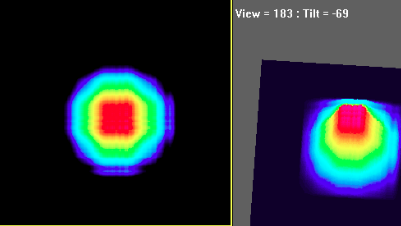
\includegraphics[scale=0.38]{rojosem.png}
						\caption{\label{Img:rojSem}Perfil del modo transversal electromagnético para el láser rojo de semiconductor.}
					\end{figure}

				En la Figura \ref{Img:rojSem} se observa un perfil poco claro por lo que no se puede determonar con precisión el modo transversal del que se trata. Esto puede ser debido a que dicho láser se haya recalentado debido al tiempo que llevaba encencido. No obstante, se sabe que debe de tratarse de un $TEM_{11}$

					\begin{figure}[H]
						\centering
						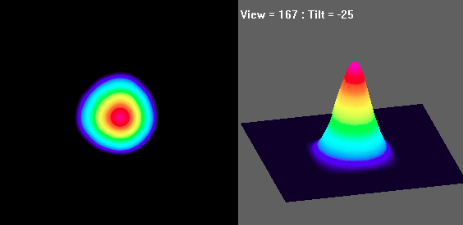
\includegraphics[scale=0.38]{rojogas.png}
						\caption{\label{Img:rojgs}Perfil del modo transversal electromagnético para el láser rojo de gas.}
					\end{figure}

				En la Figura \ref{Img:rojgs} se observa claramente el modo TEM$_{00}$ para el láser rojo de gas.

					\begin{figure}[H]
						\centering
						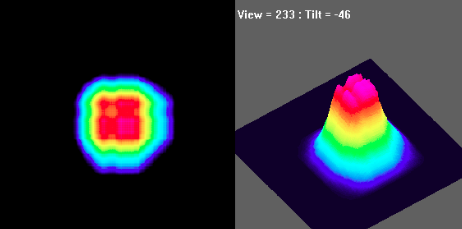
\includegraphics[scale=0.38]{azul.png}
						\caption{\label{Img:azul}Perfil del modo transversal electromagnético para el láser azul.}
					\end{figure}

				En cuanto a la Figura del láser azul \ref{Img:azul}, parece intuirse un modo $TEM_{33}$ ó un $TEM_{43}$, pero no se puede determinar con exactitud.

			\subsection{Emisión de láser}

				En la Tabla \ref{Tab:Max} se muestran los datos de la longitud de onda y el valor de la intensidad obtenidos para la máxima intensidad de cada láser.

					\begin{table}[H]
						\centering
						\begin{tabular}{c c c}
							\hline
							\centering
								Láser & $\lambda_{max} \pm 0.2 /nm$ & $I_{max} \pm 0.5 /nW$ \\ \hline
								Gas Rojo & 632.2 & 85.9 \\
								Sem Rojo & 662.2 & 96.0 \\
								Azúl & 407.2 & 12.7 \\ \hline
						\end{tabular}
						\caption{\label{Tab:Max}Longitud de onda y el valor de la intensidad obtenidos para la máxima intensidad de cada láser.}
					\end{table}

				En la Tabla \ref{Tab:media} se muestran los datos de la longitud de onda y el valor de la intensidad obtenidos para la mitad de la máxima intensidad de cada láser.

					\begin{table}[H]
						\centering
						\begin{tabular}{c c c}
							\hline
							\centering
								Láser & $\lambda_{1/2} \pm 0.2 /nm$ & $I_{1/2} \pm 0.5 /nW$ \\ \hline
								Gas Rojo & 633.0 & 44.0 \\
								Sem Rojo & 661.0 & 48.0 \\
								Azúl & 406.0 & 6.3 \\ \hline
						\end{tabular}
						\caption{\label{Tab:media}Longitud de onda y el valor de la intensidad obtenidos para la mitad de la máxima intensidad de cada láser.}
					\end{table}

				En la Tabla \ref{Tab:deltaLambda} se muestran las anchuras espectrales obtenidas de la diferencia entre $\Delta \lambda = \lambda_{max} - \lambda_{1/2}$ con los datos de las Tablas \ref{Tab:Max} y \ref{Tab:media}.

					\begin{table}[H]
						\centering
						\begin{tabular}{c c}
							\hline
							\centering
								Láser & $\Delta \lambda / nm$ \\ \hline
								Gas Rojo & 1.6 \\
								Sem Rojo & 2.4 \\
								Azúl & 2.4 \\ \hline
						\end{tabular}
						\caption{\label{Tab:deltaLambda}Anchuras espectrales obtenidas de la diferencia entre $\Delta \lambda = \lambda_{max} - \lambda_{1/2}$ con los datos de las Tablas \ref{Tab:Max} y \ref{Tab:media}.}
					\end{table}

			\subsection{Fabry-Perot}

				Se han realizado las medidas dos veces de la distancia que hay que mover los espejos para obtener dos máximos consecutivos en el centro del patrón de difracción. En la Tabla \ref{Tab:FP} se muestran dichos datos.

					\begin{table}[H]
						\centering
						\begin{tabular}{c c c c}
							\hline
							\centering
								$d_1 /$mm & $d_2 /$mm & $\Delta d /$ mm & $\lambda /$ nm\\ \hline
								17.18 & 17.45 & 0.27 & 604.8 \\
								16.92 & 16.75 & 0.17 & 380.8 \\ \hline
						\end{tabular}
						\caption{\label{Tab:FP}Distancia entre los dos espejos para el primer máximo de interferencia $d_1$, la distancia para el segundo máximo de interferencia $d_2$, la diferencia entre ambas distancias $\Delta d$ y la longitud de onda del láser incidente obtenida a partir de la ecuación \ref{eq:fp}.}
					\end{table}

				A partir de estos daots se puede obtener un valor medio de la longitud de onda del láser incidente.

					\begin{equation}
						\lambda = 490 \pm 160 nm
					\end{equation}

				Se puede observer que dicho valor obtenido para $\lambda$ no corresponde con los valores esperados para un láser de dichas características ($660-630$ nm). Esto puede deberse a que, al tratarse de distancias tan pequeñas, cualquier fluctuación en el medio puede afectar al patrón de interferencia. De esta forma, uno de los posibles efectos puede ser que no se esté midiendo exáctamente la posición para el máximo consecutivo. No obstante, el valor obtenido sí es compatible con los valores esperados debido al gran error obtenido. 

	\end{multicols}

%----------------------------------------------------------------------------
%     APPENDIX
%----------------------------------------------------------------------------

%\newpage
%
%	    \appendix
%
%	    	\section{}
%	    		\label{appen:}

	    		
	    		
%----------------------------------------------------------------------------
%     BIBLIOGRAPHY
%----------------------------------------------------------------------------

%	\bibliographystyle{unsrt}
%	\bibliography{biblio}

\end{document}


%----------------------------------------------------------------------------
%            TEMPLATES
%----------------------------------------------------------------------------

%----------------------------------------------------------------------------
%            how to insert an image
%----------------------------------------------------------------------------

%	\begin{figure}[H]
%		\centering
%		\includegraphics[scale= ]{nombre de la imagen.jpg}
%		\caption{\label{Img:widgets}el pie de pagina que le quieras 	poner a la imagen}
%	\end{figure}
 
%----------------------------------------------------------------------------
%            how to insert a table
%----------------------------------------------------------------------------

%	\begin{table}[H]
%		\centering
%		\begin{tabular}{|c|c|c|c|}
%			\hline
%			\centering
%				Altura(h) & Distancia (d) & Elaboracion (e) & Longitud (l) \\
%				($\pm0.5$ mm) & ($\pm0.5$ mm) & ($\pm0.5$ mm) & ($\pm0.5$ mm) \\ \hline
%				 &  &  &  \\ \hline
%				 &  &  &  \\ \hline
%				 &  &  &  \\ \hline
%				 &  &  &  \\ \hline
%				 &  &  &  \\ \hline
%		         &  &  &  \\ \hline
%		\end{tabular}
%		\caption{\label{Tab:widgets}pie de pagina que le quieras poner}
%	\end{table}

%----------------------------------------------------------------------------
%             How to remove the label in equactions
%----------------------------------------------------------------------------

%	\begin{equation*}
%		
%	\end{equation*}

%----------------------------------------------------------------------------
%              How to set bibliography
%----------------------------------------------------------------------------

%\bibliographystyle{unsrt}
%\bibliography{biblio}
%
%Then you have to set a .bib document such as the next template
%
%	@book{nickname,
%	author = {},
%	title = {},
%	edition = {},
%	year = {},
%	volume = {},
%	ISBN = {}
%	}
%
%	@ARTICLE{nickname,
%	author = {},
%	title = {},
%	year = {},
%	volume = {},
%	}


%----------------------------------------------------------------------------
%              END
%----------------------------------------------------------------------------
